\documentclass[a4paper]{article}
%AMDG
\usepackage{amsmath, amsthm, amssymb}
\usepackage{hyperref}
\usepackage[slovene]{babel}
\usepackage[utf8]{inputenc}
\usepackage[T1]{fontenc}
\usepackage{epigraph}
\usepackage{pdftexcmds}
\usepackage{fancyref, nameref}
\usepackage{epigraph}
\usepackage{cleveref}
\usepackage{verbatim}
\usepackage{enumitem}
\usepackage{multicol}
\usepackage[nomessages]{fp}
\usepackage{fancyhdr}
\usepackage{multirow}
\usepackage{mathtools}
\usepackage{graphicx}
\usepackage{caption}
\usepackage{subcaption}
\usepackage[justification=centering]{caption}

\usepackage{tikz}


\parindent=0pt


% \epigraphsize{\small}% Default
\setlength\epigraphwidth{8cm}
\setlength\epigraphrule{0pt}

\usepackage{etoolbox}

\makeatletter
\patchcmd{\epigraph}{\@epitext{#1}}{\itshape\@epitext{#1}}{}{}
\makeatother


\newcounter{environment:definition_counter}

\newenvironment{definition}[1][\unskip]
{\vspace{0.5cm}\refstepcounter{environment:definition_counter}\textbf{Definicija \arabic{environment:definition_counter}: \textbf{#1}}\itshape}
{\bigskip}

\newcounter{environment:theorem_counter}

\newenvironment{theorem}[1][\unskip]
{\refstepcounter{environment:theorem_counter}\textbf{Izrek \arabic{environment:theorem_counter}:\textit{#1}}\\}
{\bigskip}

\newcounter{environment:statement_counter}

\newenvironment{statement}[1][\unskip]
{\refstepcounter{environment:statement_counter}\textbf{Trditev \arabic{environment:statement_counter}:\textit{#1}}}
{\bigskip}

\newcounter{example:example_counter}

\newenvironment{example}
{\textbf{Primer:}\\}
{\setcounter{example:example_counter}{0}}

\newenvironment{example_case}
{\refstepcounter{example:example_counter} \arabic{example:example_counter}.}
{\\}

\newenvironment{remark}
{\textbf{Opomba:}}
{}

\newenvironment{corollary}
{\underline{\textbf{Posledica:}}}
{}

%should rethink this
\newtheorem{lemma}{Lema}

\newcommand{\subscript}[2]{$#1 _ #2$}

\newcommand{\twopartdef}[4]
{
	\left\{
		\begin{array}{ll}
			#1 & \mbox{; } #2 \\
			#3 & \mbox{; } #4
		\end{array}
	\right.
}


\pagestyle{headings}
\pagestyle{fancy}
%\fancyhead[LE,RO]{\itshape \nouppercase \rightmark}
%\fancyhead[LO,RE]{\itshape \nouppercase Chapter \arabic{chapter}}


\lfoot{Mreže}
\rfoot{Filip Koprivec, Samo Kralj}

%operatorji
\newcommand{\ord}{\ensuremath{\operatorname{red}}} % red grupe/elementa
\newcommand{\Mod}[1]{ \ (\text{mod}\ #1)}

\begin{document}	
\title{Mreže}
\author{Filip Koprivec, Samo Kralj}
\date{\today}
\maketitle

\epigraph{“If I find in myself desires which nothing in this world can satisfy, the only logical explanation is that I was made for another world.”}{--- \textup{C. S. Lewis}}
\newpage

\tableofcontents

\newpage

\section{Uvod}

Mreža je množica z dodatno strukturo (delno urejenostjo), ki zadošča poguju, da ima poljuben par elementov infimum in supremum. Najprej si bomo pogledali mreže s stališča matematične logike in urejenosti, kasneje pa si jih bomo ogledali še s stališča algebraičnih operacij nad njimi, ter pokazali, zakaj sta ta dva pogleda ekvivalentna.

%TODO uredi uvod

\subsection{Osnovne definicje}
\begin{definition}
Naj bo $\mathcal{L}$ množica, relacija $\leq$ je \textbf{(šibka) delna urejenost}, če je
\begin{itemize}
\item refleksivna ($a \leq a$)
\item antisimetrična ($a \leq b \land b \leq a \implies a = b$)
\item tranzitivna ($a \leq b \land b \leq c \implies a \leq c$)
\end{itemize}
Pišemo $a$ je manjši ali enak $b$, občasno tudi $a$ je pod $b$.
\end{definition}

\begin{remark}
Zgolj iz preprostosti definiramo še drugo relacijo $a \geq b \iff b \leq a$, ki je očitno tudi delna urejenost.
\end{remark}
\\
\\
\begin{remark}
Poznamo tudi \textbf{strogo delno urejenost}, ki jo definiramo kot $a < b \iff a \leq b \land a \neq b$  
\end{remark}

\begin{example}
Tipičen primer delne urejenosti je kar sama motivacija za vpeljavo relacije. Vzemimo množico realnih števil $\mathbb{R}$ in na njej relacijo $\leq$, za katero preprosto preverimo da je delna urejenost.
\end{example}
\\
\\
\begin{statement}
Relacija deljivosti ($\mid$) na množici $\mathbb{N}$ je delna urejenost.
\end{statement}
\begin{proof}
Preverili bomo da ta relacija zadošča vsem zahtevam. Spomnimo se, da $a$ deli $b$ natanko tedaj, kadar obstaja tako celo število $k$, da zadosti enakosti $b = ka$, oziroma $a \mid b \iff \exists k \in \mathbb{Z}. \ b = ka$.
\begin{itemize}
\item Refleksivnost: $a = 1*a$, torej $a \mid a$
\item Antisimetričnost: $a \mid b \implies b = k_1a$, $b \mid a \implies a = k_2b$, vstavimo $a$ v prvo enakost in dobimo $b = k_1k_2 b$, torej $k_1 = k_2^{-1}$, torej $k_1 = k_2 = 1$ in dobimo $b = a$
\item Tranzitivnost: $a \mid b \land b \mid c \implies a \mid c$, vemo torej $b = k_1a$ in $c = k_2b$, vstavimo prvo enakost v drugo in dobimo $c = \underbrace{k_2k_1}_{\in \mathbb{Z}}a$ torej $a \mid c$.
\end{itemize}
\end{proof}

\begin{remark}
Preprosto preverimo, da je za poljubno množico $\mathcal{A}$, relacija $\subseteq$ delna urejenost na potenčni množici množice $\mathcal{A}$ ($P(\mathcal{A})$).
\end{remark}

\begin{definition}
Množica $\mathcal{L}$ je \textbf{linearno urejena}, če za poljubna $x,y$ velja $x \leq y$ ali  $y \leq x$ 
\end{definition}

\begin{example}
Množica $\mathbb{N}$ z urejenostjo $\leq$ je linearno urejena, saj za poljubna $x$ in $y$ velja $x \leq y \lor y \leq x$, če pa velja $x=y$, potem pa sta pravilna celo oba dela izjave. Množica $\mathbb{N}$ urejena glede na relacijo deljivosti pa \textbf{ni} linearno urejena, saj za recimo dve poljubni praštevilo velja $p_1 \nmid p_2 \land p_2 \nmid p_1$.
\end{example}
\\
\begin{remark}
Pridstavitem linearno urejenih množic s Hassejevim diagramom nas spominja na premico, od torej tudi izraz. To je lepo vidno na sliki (\ref{im:natural_numbers_hasse_example}).
\end{remark}
\\
Za lepšo predstavo splošnih linearnih urejenih diagramov si pomagamo s Hassejevim diagramom, ki s pomočjo povezav med točkami prikaže relacije med njimi.

\begin{definition}
Naj bo $\mathcal{L}$ delno urejena množica glede na neko relacijo, ki o označimo z $\leq$. Hassejev diagram je graf, katerega točke so elementi $\mathcal{L}$, med točkama $x$ in $y$ pa je povazava natnko tedaj, kadar velja: $$ x \leq y \land \nexists z \in \mathcal{L}. \ x \leq z \leq y$$
\end{definition}

\begin{figure}[h]
  \begin{subfigure}[b]{0.1\textwidth}
    \begin{tikzpicture}
      \node (a) at (0,0) {};
      \node (c) at (0,-2) {$2$};
      \node (d) at (0,-3) {$1$};
      \node (e) at (0,-4) {$0$};
      \draw  (c) -- (d) -- (e);
      \draw[dotted] (c) -- (a);
    \end{tikzpicture}
    \caption{$\mathbb{N}, \leq$}
    \label{im:natural_numbers_hasse_example}
  \end{subfigure}  
  \hfill
  \begin{subfigure}[b]{0.8\textwidth}
\begin{tikzpicture} % should make python program :(
  \node (one) at (1,4) {$0$};
  \node (two) at (-3,0) {$2$};
  \node (three) at (-1,0) {$3$};
  \node (five) at (2,0) {$5$};
  \node (rest_primes) at (4,0) {$\dots$};
  \node (rest_primes_2) at (5,0) {$\dots$};
  \node (rest_second) at (4,2) {$\dots$};
  \node (rest_second_2) at (5,2) {$\dots$};
  
  \node (four) at (-3,2) {$4$};
  \node (six) at (-2,2) {$6$};
  \node (nine) at (-1,2) {$9$};
  \node (ten) at (0,2) {$10$};
  \node (fifteen) at (1, 2) {$15$};
  \node (twentyfive) at (2,2) {$25$};
  
  \node (zero) at (1,-2) {$1$};
  
  \draw (zero) -- (two) -- (six) -- (three) -- (fifteen) -- (five) -- (zero) -- (rest_primes);
  \draw (rest_primes_2) -- (zero) -- (three);


  \draw (two) -- (four);
  \draw (three) -- (nine);
  \draw (two) -- (ten) -- (five);
  \draw (five) -- (twentyfive);
  \draw[loosely dotted] (four) -- (one);  
  \draw[loosely dotted] (six) -- (one);  
  \draw[loosely dotted] (nine) -- (one);  
  \draw[loosely dotted] (ten) -- (one);
  \draw[loosely dotted] (fifteen) -- (one);  
  \draw[loosely dotted] (twentyfive) -- (one);  
  \draw[loosely dotted] (rest_primes) -- (rest_second) -- (one);
  \draw[loosely dotted] (rest_primes_2) -- (rest_second_2) -- (one);
  
\end{tikzpicture}
  \caption{Hassejev diagram za $(\mathbb{N}, \mid)$}
  \label{im:natural_nubmers_divisibility_hasse_example}
  \end{subfigure}
\caption{Primer Hassejevih diagramov}
\label{im:hasse_diagram_example}
  \end{figure}

\subsection{Supremum in infimum}



\begin{definition}
$S$ je \textbf{supremum} $x$ in $y$, če velja: 
\begin{itemize}
\item $S \geq x \land S \geq y$ (Zgornja meja)
\item $\forall S' \in \mathcal{L} \implies (S' \geq x \land S' \geq y \implies S \leq S')$ (Je najmanjša zgornja meja)
\end{itemize}
Torej je $S$ natačna zgornja meja $x$ in $y$, če je njuna zgornja meja, hkrati pa je vsaka od $S$ različna zgornja meja večja ali enaka $S$. Označimo: $S = x \lor y$. 
\end{definition}


\begin{definition}
$s$ je \textbf{infimum} $x$ in $y$, če velja: 
\begin{itemize}
\item $s \leq x \land s \leq y$ (Spodnja meja)
\item $\forall s' \in \mathcal{L} \implies (s' \leq x \land s' \leq y \implies s' \leq s)$ (Je največja spodnja meja)
\end{itemize}
Torej je $s$ natačna spodnja meja $x$ in $y$, če je njuna spodnja meja, hkrati pa je vsaka od $s$ različna zgornja meja manjša ali enaka $s$. Označimo: $s = x \land y$ .
\end{definition}

\begin{remark}
V literaturi se za supremum občasno uporablja tudi oznaka $\cup$, za infimum pa $\cap$. 
\end{remark}

\begin{example}
\begin{example_case}
Za množico $\mathbb{R}$, ki je urejena glede na $\leq$ in poljubni števili $x,y$ velja: $x \lor y = max\{x,y\}$ in $x \land y = min\{x,y\}$.
\end{example_case}
\begin{example_case}
Za množico $\mathbb{N}$, ki je urejena glede na relacijo deljivosti in poljubni števili $x,y$ velja: $x \lor y = lcm\{x,y\}$ (najmanjši skupni večkratnik) in $x \land y = gcd\{x,y\}$ (največji skupni delitelj).
\end{example_case}
\end{example}

\subsection{Definicja mreže}

\begin{definition}
Množica $\mathcal{L}$ je \textbf{mreža}, če za poljuben par $x,y$ v $\mathcal{L}$ obstajata infimum in supremum.
\end{definition}

\begin{example}
Naravna števila so mreža tako za urejenost glede na relacijo $\leq$, kot tudi za urejenost glede na relacijo deljivosti. To lahko lepo vidimo na sliki (\ref{im:hasse_diagram_example}). 
\end{example}

\begin{definition}
Mreža $\mathcal{L}$ je polna, če za poljubno $\mathcal{A} \subseteq \mathcal{L}$ obstajata infimum in supremum za $\mathcal{A}$.
\end{definition}

\begin{example}
Poljubna končna mreža je tudi polna mreža. Preprosto za infumum in supremum vzamemo infimum in supremum elementov po parih. Na podoben način pa dobimo mreže, ki niso polne. $\mathbb{R}, \leq$ ni polna, saj množica $\mathbb{N}$ nima niti infimuma niti supremuma.
\end{example}

\section{Osnovni primeri mrež}

Od prej se spomnimo, je poljubna podmnožica $\mathbb{R}$, urejena glede na relacijo $\leq$ mreža. Za poljubni števili $x,y$ velja: $x \lor y = max\{x,y\}$ in $x \land y = min\{x,y\}$, seveda pa sta tako infimum kot supremum v mreži. Opazimo, da so te množice vedno liearno urejene.
\\\\
Množica naravnih števil pa nam poleg urejenosti z $\leq$ omogoča tudi ureditev z $\mid$. V tem primeru dobima Hassejev diagram iz slike (\ref{im:natural_nubmers_divisibility_hasse_example}). Ta množica nima liearne ureditve, opazimo, pa da elementa $0$ in $1$ na nek način zaključujeta mrežo, saj so vsa naravna števila pod $0$ (delijo $0$), hkrati pa $1$ deli vsa ostala naravna števila. S slike tudi lepo opazimo, da s v prvem nivoju urejenosti samo preštevila, v drugem nivoju urejenosti števila z natančno dvema deliteljema in v $n$-tem, nivoju ptevila z $n$ delitelji.
\\\\
\begin{remark}
Če v naravna števila vključimo tudi $0$, potem formula za supremum in infimum glede na najmanjše skupne večkratnike in največje skupne delitelje ne deluje več kadar je eden izmed argumentov $0$.
\end{remark}

\begin{figure}
\centering
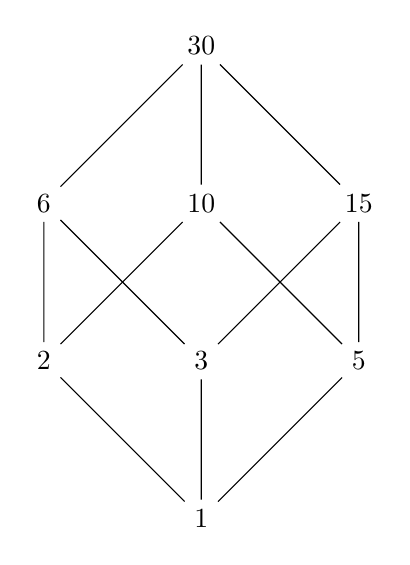
\begin{tikzpicture}
  \node (one) at (0,0) {$30 $};
  \node (two) at (-2,-4) {$2 $};
  \node (three) at (0,-4) {$3 $};
  \node (five) at (2,-4) {$5 $};
  
  \node (four) at (-2,-2) {$6 $};
  \node (six) at (0,-2) {$10 $};
  \node (nine) at (2,-2) {$15 $};
  
  \node (zero) at (0,-6) {$1 $};
  
  \draw (zero) -- (two) -- (four) -- (one) -- (six) -- (two);  
  \draw (zero) -- (three) -- (four);
  \draw (zero) -- (five) -- (six);
  \draw (three) -- (nine);
  \draw (one) -- (nine) -- (five);
\end{tikzpicture}
\caption{Mreža deliteljev števila $15$ urejena glede na relacijo deljivosti}
\label{im:divisors_of_30_hasse_diagram}
\end{figure}

Pomembne mreže pa predstavljajo tudi mreže deliteljev posameznega naravnega števila. To lepo vidmo na sliki (\ref{im:divisors_of_30_hasse_diagram}).

Delno urejene množice lahko predstavimo zgolj s Hassejevim diagramom. Poglejmo si nekaj množic, ki niso mreže in razložimo zakaj ne.

\begin{figure}[h]
  \begin{subfigure}[h]{0.3\textwidth}
  \centering
  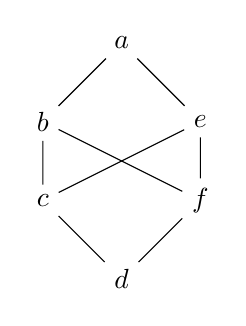
\begin{tikzpicture}
    \node (a) at (0,0) {$a$};
    \node (b) at (-1,-1) {$b$};
    \node (c) at (-1,-2) {$c$};
    \node (d) at (0,-3) {$d$};
    \node (e) at (1,-1) {$e$};
    \node (f) at (1,-2) {$f$};
    \draw (a) -- (b) -- (c) -- (d) -- (f) -- (e) -- (a);
    \draw (f) -- (b);
    \draw (c) -- (e);
  \end{tikzpicture}
    \caption{Delno urejena množica, ki ni mreža}
    \label{im:not_lattice_1}
  \end{subfigure}  
  \hfill
  \begin{subfigure}[h]{0.3\textwidth}
  \centering
  \begin{tikzpicture}
    \node (a) at (0,0) {$a$};
    \node (b) at (-1,-1) {$b$};
    \node (c) at (-1,-2) {$c$};
    \node (d) at (0,-3) {$d$};
    \node (e) at (1,-1.5) {$e$};
    \node (f) at (1.5,-2.5) {$f$};
    \draw (a) -- (b) -- (c) -- (d) -- (e) -- (a);
    \draw (e) -- (f);
  \end{tikzpicture}
  \caption{$\{a,b,c,d,e,f\}$, ni mreža}
  \label{im:not_lattice_2}
  \end{subfigure}
  \hfill
  \begin{subfigure}[h]{0.3\textwidth}
  \centering
  \begin{tikzpicture}
    \node (a) at (0,0) {$12$};
    \node (b) at (-1,-1) {$4$};
    \node (c) at (-1,-2) {$2$};
    \node (d) at (0,-3) {$1$};
    \node (e) at (1,-1.5) {$3$};
    \draw (a) -- (b) -- (c) -- (d) -- (e) -- (a);
  \end{tikzpicture}
  \caption{$(\{1,2,3,4,6\}, |)$, je mreža}  
  \label{im:divisors_of_6_lattice}
  \end{subfigure}

\caption{Primer delno urejenih množic, ki niso mreže}
\label{im:not_lattice_example}
  \end{figure}

Če si pogledamo sliko (\ref{im:not_lattice_example}) lahko hitro vidimo, zakaj te množici nista mreži. Množica na sliki (\ref{im:not_lattice_1}) ni mreža, saj elementa $c$ in $f$ nimata natančno določenega supremuma. Vidimo, da bi to lahko bila tako element $e$ kot tudi element $b$, vendar pa ju med samo ne moremo primerjati. Množica na sliki (\ref{im:not_lattice_1}) zato ni mreža. Bi pa postala mreža, če bi odstranili povezamo med $c$ in $e$.
\\\\
Če pa pogledamo sliko (\ref{im:not_lattice_2}) vidimo, da je problematičen element $f$. Tako recimo elementa $c \lor f = a$, medtem, ko je $c \land f$ nedoločen in zato množica ni mreža, bi pa to postala, če bi iz nje odstranili element $f$ in tako dobili mrežo vseh deliteljev števila $12$. 
\\\\
\begin{figure}
\centering
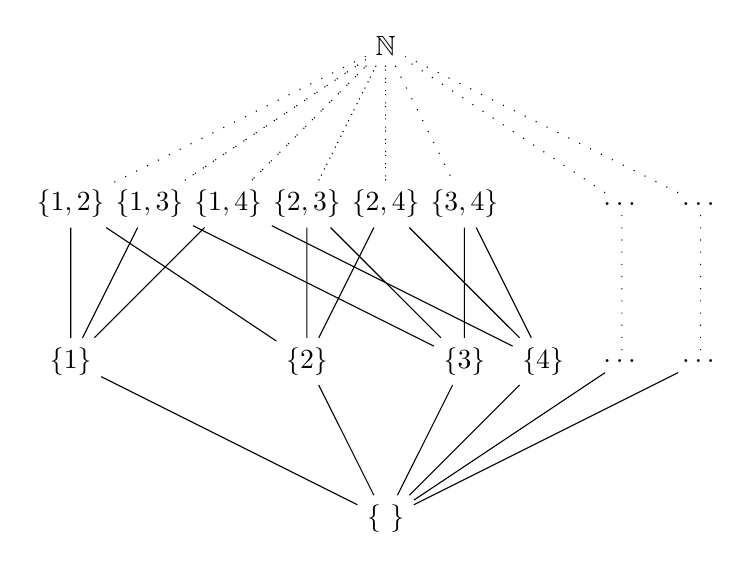
\begin{tikzpicture} % should make python program :(
  \node (one_s) at (1,4) {$\mathbb{N}$};
  \node (one) at (-3,0) {$\{1\}$};
  \node (two) at (0,0) {$\{2\}$};
  \node (three) at (2,0) {$\{3\}$};
  \node (four) at (3,0) {$\{4\}$};
  \node (rest_single) at (4,0) {$\dots$};
  \node (rest_single_2) at (5,0) {$\dots$};
  \node (rest_pair) at (4,2) {$\dots$};
  \node (rest_pair_2) at (5,2) {$\dots$};
  
  \node (one_two) at (-3,2) {$\{1,2\}$};
  \node (one_three) at (-2,2) {$\{1,3\}$};
  \node (one_four) at(-1,2) {$\{1,4\}$};
  \node (two_three) at (0,2) {$\{2,3\}$};
  \node (two_four) at (1,2) {$\{2,4\}$};
  \node (three_four) at (2,2) {$\{3,4\}$};
  
  \node (zero) at (1,-2) {$\{ \ \}$};
  
  \draw (zero) -- (one) -- (one_two) -- (two);
  \draw (zero) -- (two) -- (two_three) -- (three);
  \draw (zero) -- (three) -- (three_four) -- (four) -- (zero);
  \draw (zero) -- (rest_single);
  \draw (zero) -- (rest_single_2);	
	
  
  \draw (one) -- (one_three);
  \draw (one) -- (one_four);
  \draw (two) -- (two_four);
  \draw (three) -- (one_three);
  \draw (four) -- (one_four);
  \draw (four) -- (two_four);  
  

  \draw[loosely dotted] (one_two) -- (one_s) -- (one_three) -- (one_s) -- (one_four) -- (one_s) -- (two_three) -- (one_s) -- (two_four) -- (one_s) -- (three_four);

  \draw[loosely dotted] (rest_single) -- (rest_pair) -- (one_s);
  \draw[loosely dotted] (rest_single_2) -- (rest_pair_2) -- (one_s);
  
\end{tikzpicture}
\caption{Hassejev diagram za $\mathcal{P}(\mathbb{N}), \subseteq$}
\label{im:hasse_diagram_natural_subset}
\end{figure}

Pomemben primer mreže je tudi potenčna množica poljubne množice urejena glede na relacijo inkluzije ($\subseteq$), to lepo vidimo na sliki (\ref{im:hasse_diagram_natural_subset}). Da se prepričamo, da je ta množica mreža, preprosto preverimo supremume in infimume. 

Vidimo, da velja $x \lor y = x \cup y$ in $x \land y = x \cap y$, kar nam pojasni, zakaj se občasno za označevanje supremuma in infimuma uporablja oznaki $\cap, \cup$, saj naravno sledita iz potenčne množice kot mreže.

Takoj opazimo, da je tako kot mreža $(\mathbb{N}, \mid)$ tudi ta mreža omejena, saj je $\{\}$ pod vsemi ostalimi, $\mathbb{N}$ pa nad vsemi. Prav tako pa vidimo da v $n$ tem nivoju nastopajo vse možne $n$-elementne podmnožice začetne množice.
\\\\
\begin{remark}
Če bi za mrežo vzeli potenčno množico kakšne končne množice bi lahko s pomočjo kombinatorike lepo prešteli število množic v posameznem nivoju. Tako je za množico moči $n$ v $k$-tem nivoju $\binom {n}{k}$ elementov. Seštevek množic po vseh nivojih pa ravno $2^n$, torej ravno moč potenčne množice.
\end{remark}

\section{Zakoni v mrežah}

Mreže smo si do sedaj pogledali s stališča linearne urejenosti, kmalu pa bomo videli tudi, da lahko zgolj iz nekaterih zakonov, ki veljajo za infimume in supremume na poljubni množici za to množico dobimo delno urejenost in tako iz množice skupaj s temi zakoni tudi mrežo.
\\
\\
\begin{theorem}
Za poljubno mrežo $\mathcal{L}$ in poljubne $x,y,z \in \mathcal{L}$ veljajo naslednji zakoni:
\begin{itemize}
\item $x \lor x = x$, $x \land x = x$ (Idempotentnost)
\item $x \lor y = y \lor x$, $x \land y = y \land x$ (Komutativnost)
\item $(x \lor y) \lor z = x \lor (y \lor z)$\\ $(x \land y) \land z = x \land (y \land z)$ (Asociativnost)
\item $ x \lor (x \land y) = x$\\ $x \land (x \lor y) = x$ (Absorbcija)
\end{itemize}
\end{theorem}

\begin{proof}\leavevmode
\begin{itemize}
\item Idempotentnost: Zaradi relfeksivnosti velja $x \leq x$ in je torej tako zgornja kot spodnja meja $x, x$, prav tako pa so vse ostale spodnje ali zgornje meje manjše ali večje od $x$.
\item Komutativnost: Preprosto sledi iz definicije, saj je meja neodvisna od vrstnega reda elementov
\item Asociativnost: Preverimo za $\lor$: \\
Naj bo $a = (x \lor y) \lor z$ in $b = x \lor (y \lor z)$ \\ 
Iz definicje ali sledi $a \geq z$ in $a \geq (x \lor y)$ in torej $a \geq x, a \geq y$ \\ 
Potem velja tudi $a \geq (y \lor z)$ in $a \geq x \lor (y \lor z)$ torej $a \geq b$\\ 
Podobno postopamo za nasprotno stran in tako dobimo $b \geq a$, ker pa je zaradi antisimetričnosti relacije mogoče zgolj, kadar velja $a=b$\\
Na analogen način preverimo tudi za $\land$, samo da $a$ in $b$ omejimo navzgor.
\item Absorbcija: Preverimo za $x \land (x \lor y) = x$:\\
Iz definicije $\lor$ vemo $x \leq (x \lor y)$ in $x \leq x$ torej $x \leq x \land (x \lor y)$\\ 
Iz definicije $\land$ pa sledi $x \geq x \land (x \lor y)$\\
Torej $x \leq x \land (x \lor y)$ in $x \geq x \land (x \lor y)$, dobimo $x = x \land (x \lor y)$\\
Drugo enakost preverimo analogno.
\end{itemize}
\end{proof}

Pomembno ugotovitev pa nam prinaša naslednji izrek, ki nam pove, da sta si ta dva pogoja za mrežo ekvivalentna.
\\
\\
\begin{theorem}
Če imamo množico $\mathcal{L}$, za katero sta definirani operaciji $\lor, \land$ in če za te dve operacji veljajo zgornji zakoni(idempotentnost, komutativost, asociativnost, absorbcija), potem je ta množica mreža.
\end{theorem}

\begin{proof}
Najprej si s pomočjo supremuma in infimuma definirajo relacijo delne urejenosti.\\
Definiramo: $x \leq y \iff x \land y = x$ in preverimo, da to ustreza zahtevam delne urejenosti:
\begin{itemize}
\item Refleksivnost: $x \land x = x \implies x \leq x$
\item Antisimetričnost: $x \leq y$ in $y \leq x$, torej $x \land y = x$ in $y \land x = y$, uporabimo komutativnost in dobimo $x = y$
\item Tranzitivnost: $x \leq y$ in $y \leq z$ torej velja $x = x \land y$ in $y = y \land z$ \\ Namesto $y$ uporabimo $y \land z$ in dobimo $x = x \land (y \land z) = (x \land y) \land z = x \land z$ torej  $x \leq z$\\
Da ustreza relaciji na mreži moramo preveriti še da velja: $x \land y = x \iff x \lor y = y$:\\ 
Uporabimo zadnji zakon in dobimo $x \lor y = (x \lor y) \land y = y$, v drugo smer pa postopamo identično.
\end{itemize}
\end{proof}

\end{document}
